\documentclass[11pt,a4paper]{article}

% Packages
\usepackage[utf8]{inputenc}
\usepackage[T1]{fontenc}
\usepackage{amsmath,amssymb,amsfonts}
\usepackage{graphicx}
\usepackage{booktabs}
\usepackage{longtable}
\usepackage{hyperref}
\usepackage{xcolor}
\usepackage{geometry}
\usepackage{fancyhdr}
\usepackage{listings}
\usepackage{tcolorbox}
\usepackage{enumitem}
\usepackage{tikz}
\usetikzlibrary{shapes,arrows,positioning}

% Page setup
\geometry{margin=1in}
\pagestyle{fancy}
\fancyhf{}
\rhead{A/B Testing Methodology}
\lhead{Optimized Checkout}
\rfoot{Page \thepage}

% Colors
\definecolor{primaryblue}{RGB}{41,128,185}
\definecolor{successgreen}{RGB}{39,174,96}
\definecolor{warningorange}{RGB}{230,126,34}
\definecolor{dangerred}{RGB}{192,57,43}
\definecolor{codegray}{RGB}{245,245,245}

% Code listing style
\lstset{
    backgroundcolor=\color{codegray},
    basicstyle=\ttfamily\small,
    breaklines=true,
    frame=single,
    numbers=left,
    numberstyle=\tiny\color{gray},
    keywordstyle=\color{primaryblue},
    commentstyle=\color{successgreen},
    stringstyle=\color{warningorange},
}

% Custom boxes
\newtcolorbox{keyinsight}{
    colback=primaryblue!10,
    colframe=primaryblue,
    title=Key Insight,
    fonttitle=\bfseries
}

\newtcolorbox{warningbox}{
    colback=warningorange!10,
    colframe=warningorange,
    title=Warning,
    fonttitle=\bfseries
}

\newtcolorbox{decisionbox}{
    colback=successgreen!10,
    colframe=successgreen,
    title=Decision Rule,
    fonttitle=\bfseries
}

% Title
\title{
    \vspace{-1cm}
    {\Large\bfseries A/B Testing Methodology}\\[0.5em]
    {\large Optimized Checkout Feature}\\[1em]
    {\normalsize Integrating Statistical Rigor with Psychological Insights}
}
\author{
    Statistics Agent \and Psychology Agent \and Product Manager Agent
}
\date{January 2026 \\ Version 1.0}

\begin{document}

\maketitle
\thispagestyle{empty}

\begin{abstract}
This document defines a comprehensive A/B testing methodology for the Optimized Checkout feature, incorporating sequential testing with early-stopping strategies, psychological considerations for novelty effects and cognitive biases, and practical guardrails for safe experimentation. The methodology is grounded in research on decision-making (Bechara, 2005) and cognitive load theory (Sweller, 1988).
\end{abstract}

\tableofcontents
\newpage

%==============================================================================
\section{Executive Summary}
%==============================================================================

This methodology addresses three critical aspects of experimentation:

\begin{enumerate}
    \item \textbf{Statistical Rigor:} Group sequential design with O'Brien-Fleming spending function for valid early stopping
    \item \textbf{Psychological Validity:} Burn-in periods and segmentation to account for novelty effects and cognitive biases
    \item \textbf{Operational Safety:} Guardrail metrics and automatic rollback criteria
\end{enumerate}

\begin{keyinsight}
Key decisions:
\begin{itemize}
    \item Minimum 2-week burn-in before stopping decisions
    \item Sequential testing with 4 interim analyses
    \item Segment analysis by user behavior patterns
    \item Automatic rollback if guardrail metrics breach thresholds
\end{itemize}
\end{keyinsight}

%==============================================================================
\section{Experiment Design}
%==============================================================================

\subsection{Hypothesis}

\begin{align}
    H_0&: \pi_{\text{treatment}} = \pi_{\text{control}} \quad \text{(no effect)} \\
    H_1&: \pi_{\text{treatment}} > \pi_{\text{control}} \quad \text{(treatment improves conversion)}
\end{align}

Where $\pi$ represents the checkout conversion rate.

\subsection{Sample Size Calculation}

For a two-proportion z-test with:
\begin{itemize}
    \item Baseline conversion rate: $p_1 = 0.025$ (2.5\%)
    \item Minimum Detectable Effect: 10\% relative lift $\rightarrow p_2 = 0.0275$
    \item Significance level: $\alpha = 0.05$ (two-tailed)
    \item Statistical power: $1 - \beta = 0.80$
\end{itemize}

The required sample size per arm is:

\begin{equation}
n = \frac{2 \cdot (Z_{\alpha/2} + Z_{\beta})^2 \cdot \bar{p}(1-\bar{p})}{(p_1 - p_2)^2}
\end{equation}

Where:
\begin{itemize}
    \item $Z_{\alpha/2} = 1.96$ for $\alpha = 0.05$
    \item $Z_{\beta} = 0.84$ for power $= 0.80$
    \item $\bar{p} = (p_1 + p_2)/2 = 0.02625$
\end{itemize}

\begin{equation}
n \approx \frac{2 \cdot (1.96 + 0.84)^2 \cdot 0.02625 \cdot 0.97375}{(0.0025)^2} \approx 25{,}000 \text{ per arm}
\end{equation}

\begin{decisionbox}
\textbf{Required Sample:} $\sim$50,000 unique checkout sessions (25,000 per arm)
\end{decisionbox}

\subsection{Traffic Allocation Strategy}

\begin{table}[h]
\centering
\begin{tabular}{@{}lccc@{}}
\toprule
\textbf{Phase} & \textbf{Control} & \textbf{Treatment} & \textbf{Duration} \\
\midrule
Beta & 95\% & 5\% & 2 weeks \\
Limited & 75\% & 25\% & 2 weeks \\
Expanded & 50\% & 50\% & 2 weeks \\
Decision & \multicolumn{2}{c}{Based on results} & -- \\
\bottomrule
\end{tabular}
\caption{Phased rollout traffic allocation}
\end{table}

\subsection{Randomization Strategy}

\begin{itemize}
    \item \textbf{Randomization unit:} User ID (cookie-based for guests, account ID for logged-in users)
    \item \textbf{Stratification factors:} Device type, new vs. returning customer, geographic region
    \item \textbf{Sticky assignment:} Users remain in the same variant for the experiment duration
\end{itemize}

%==============================================================================
\section{Metrics Framework}
%==============================================================================

\subsection{Primary Metric}

\begin{table}[h]
\centering
\begin{tabular}{@{}lll@{}}
\toprule
\textbf{Metric} & \textbf{Definition} & \textbf{Success Threshold} \\
\midrule
Checkout Conversion Rate & Orders / Checkout Sessions & $\geq$10\% relative lift, $p < 0.05$ \\
\bottomrule
\end{tabular}
\caption{Primary success metric}
\end{table}

\subsection{Secondary Metrics}

\begin{table}[h]
\centering
\begin{tabular}{@{}lll@{}}
\toprule
\textbf{Metric} & \textbf{Definition} & \textbf{Expected Direction} \\
\midrule
Cart abandonment rate & Abandoned / Started checkouts & Decrease \\
Average checkout time & Time from cart to order & Decrease \\
Average order value & Revenue / Orders & Neutral or increase \\
Customer satisfaction & Post-checkout survey score & Increase \\
\bottomrule
\end{tabular}
\caption{Secondary metrics}
\end{table}

\subsection{Guardrail Metrics}

\begin{warningbox}
If \textbf{any} guardrail metric breaches its threshold, the experiment must be paused or stopped immediately.
\end{warningbox}

\begin{table}[h]
\centering
\begin{tabular}{@{}lll@{}}
\toprule
\textbf{Metric} & \textbf{Threshold} & \textbf{Action} \\
\midrule
Page load time (p95) & $> 3$ seconds & Pause experiment \\
JavaScript error rate & $> 1\%$ & Pause experiment \\
Payment failure rate & $> 2\%$ & \textcolor{dangerred}{\textbf{Stop experiment}} \\
Customer support tickets & $> 20\%$ increase & Investigate \\
Revenue per visitor & $> 5\%$ decrease & \textcolor{dangerred}{\textbf{Stop experiment}} \\
\bottomrule
\end{tabular}
\caption{Guardrail metrics and action thresholds}
\end{table}

%==============================================================================
\section{Early Stopping Strategy}
%==============================================================================

\subsection{The Peeking Problem}

Continuously monitoring A/B test results inflates the false positive rate:

\begin{warningbox}
\textbf{Example:} Checking daily for 30 days at $\alpha = 0.05$\\
Actual Type I error rate: $\sim$15--20\% (not 5\%)
\end{warningbox}

\textbf{Solution:} Use sequential testing methods that control the overall Type I error rate across multiple analyses.

\subsection{Group Sequential Design with O'Brien-Fleming Boundaries}

We employ the \textbf{O'Brien-Fleming spending function}, which is conservative early and permissive late:

\begin{equation}
\alpha^*(t) = 2 \cdot \left[1 - \Phi\left(\frac{Z_{\alpha/2}}{\sqrt{t}}\right)\right]
\end{equation}

Where:
\begin{itemize}
    \item $t$ = information fraction (proportion of total sample collected)
    \item $\Phi$ = standard normal CDF
    \item $Z_{\alpha/2} = 1.96$ for $\alpha = 0.05$
\end{itemize}

\subsection{Interim Analysis Schedule}

\begin{table}[h]
\centering
\begin{tabular}{@{}ccccc@{}}
\toprule
\textbf{Analysis} & \textbf{Info. Fraction} & \textbf{Cumulative $\alpha$} & \textbf{Z-boundary} & \textbf{p-value boundary} \\
\midrule
1st (25\%) & 0.25 & 0.0001 & 4.05 & 0.00005 \\
2nd (50\%) & 0.50 & 0.0052 & 2.80 & 0.0051 \\
3rd (75\%) & 0.75 & 0.0184 & 2.28 & 0.0226 \\
Final (100\%) & 1.00 & 0.0500 & 2.02 & 0.0431 \\
\bottomrule
\end{tabular}
\caption{O'Brien-Fleming efficacy boundaries}
\end{table}

\begin{keyinsight}
\textbf{Interpretation:}
\begin{itemize}
    \item At 25\% sample: Only stop if $p < 0.00005$ (very strong evidence required)
    \item At 50\% sample: Stop if $p < 0.0051$
    \item At 75\% sample: Stop if $p < 0.0226$
    \item At 100\%: Stop if $p < 0.0431$
\end{itemize}
\end{keyinsight}

\subsection{Futility Stopping}

Stop for futility when the conditional power falls below 10\%:

\begin{equation}
\text{Conditional Power} = P(\text{reject } H_0 \text{ at end} \mid \text{current data})
\end{equation}

\begin{table}[h]
\centering
\begin{tabular}{@{}cc@{}}
\toprule
\textbf{Analysis} & \textbf{Z-statistic for Futility} \\
\midrule
1st (25\%) & $< -0.5$ \\
2nd (50\%) & $< 0.0$ \\
3rd (75\%) & $< 0.5$ \\
\bottomrule
\end{tabular}
\caption{Futility boundaries}
\end{table}

If the observed Z-statistic falls below the futility boundary, stop the experiment and conclude no meaningful effect.

\subsection{Stopping Decision Flowchart}

\begin{figure}[h]
\centering
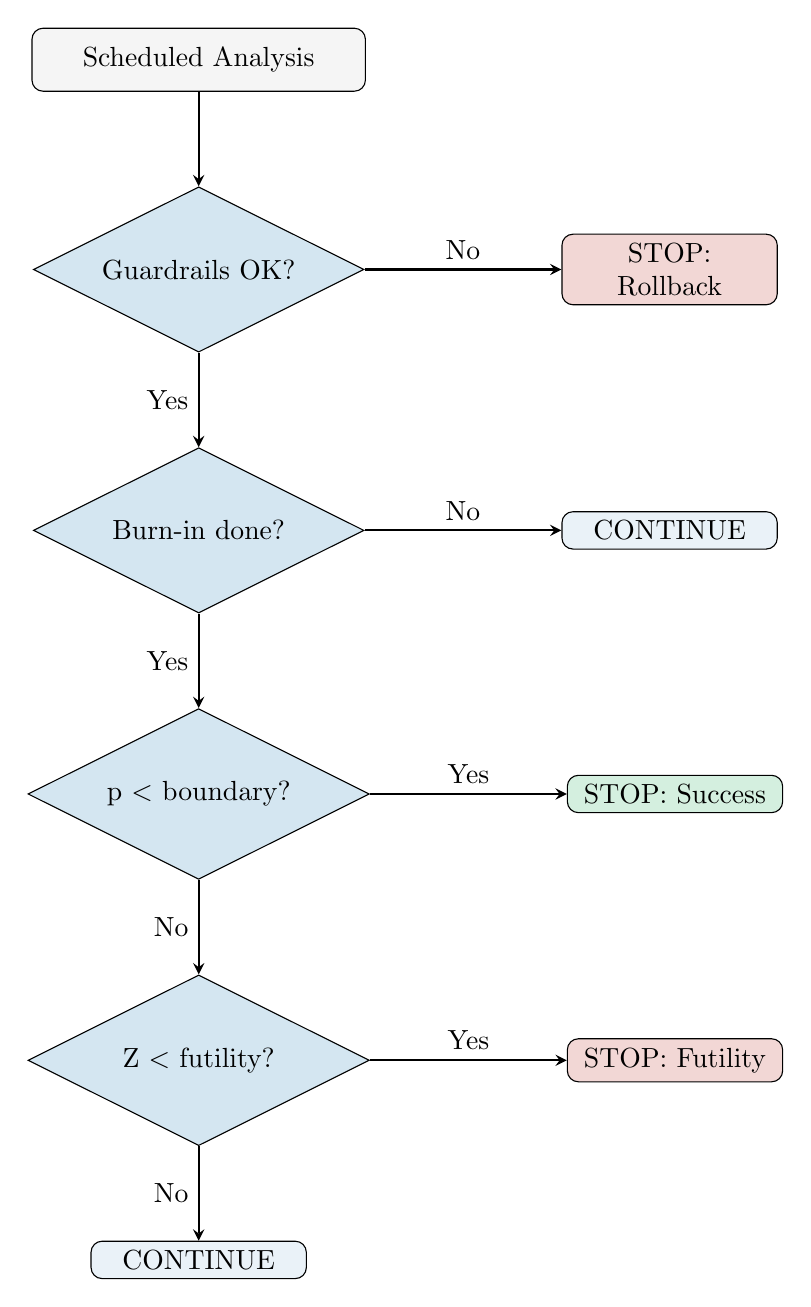
\begin{tikzpicture}[
    node distance=1.2cm,
    decision/.style={diamond, draw, fill=primaryblue!20, text width=3.5cm, text centered, inner sep=1pt, aspect=2},
    block/.style={rectangle, draw, fill=codegray, text width=4cm, text centered, rounded corners, minimum height=0.8cm},
    stop/.style={rectangle, draw, fill=dangerred!20, text width=2.5cm, text centered, rounded corners},
    success/.style={rectangle, draw, fill=successgreen!20, text width=2.5cm, text centered, rounded corners},
    continue/.style={rectangle, draw, fill=primaryblue!10, text width=2.5cm, text centered, rounded corners},
    arrow/.style={thick,->,>=stealth}
]

\node[block] (start) {Scheduled Analysis};
\node[decision, below=of start] (guardrail) {Guardrails OK?};
\node[stop, right=2.5cm of guardrail] (stop1) {STOP: Rollback};
\node[decision, below=of guardrail] (burnin) {Burn-in done?};
\node[continue, right=2.5cm of burnin] (cont1) {CONTINUE};
\node[decision, below=of burnin] (efficacy) {p $<$ boundary?};
\node[success, right=2.5cm of efficacy] (stop2) {STOP: Success};
\node[decision, below=of efficacy] (futility) {Z $<$ futility?};
\node[stop, right=2.5cm of futility] (stop3) {STOP: Futility};
\node[continue, below=of futility] (cont2) {CONTINUE};

\draw[arrow] (start) -- (guardrail);
\draw[arrow] (guardrail) -- node[above] {No} (stop1);
\draw[arrow] (guardrail) -- node[left] {Yes} (burnin);
\draw[arrow] (burnin) -- node[above] {No} (cont1);
\draw[arrow] (burnin) -- node[left] {Yes} (efficacy);
\draw[arrow] (efficacy) -- node[above] {Yes} (stop2);
\draw[arrow] (efficacy) -- node[left] {No} (futility);
\draw[arrow] (futility) -- node[above] {Yes} (stop3);
\draw[arrow] (futility) -- node[left] {No} (cont2);

\end{tikzpicture}
\caption{Stopping decision flowchart}
\end{figure}

\subsection{Bayesian Alternative}

For teams preferring Bayesian methods:

\begin{align}
\text{Prior:} & \quad \text{Beta}(1, 1) \text{ (uninformative)} \\
\text{Posterior:} & \quad \text{Beta}(\alpha + \text{successes}, \beta + \text{failures})
\end{align}

\begin{decisionbox}
\textbf{Bayesian Decision Rules:}
\begin{itemize}
    \item Stop for efficacy: $P(\pi_{\text{treatment}} > \pi_{\text{control}} \mid \text{data}) > 0.99$
    \item Stop for futility: $P(\pi_{\text{treatment}} > \pi_{\text{control}} \mid \text{data}) < 0.10$
    \item Continue: Otherwise
\end{itemize}
\end{decisionbox}

%==============================================================================
\section{Psychological Considerations}
%==============================================================================

\subsection{Novelty and Habituation Effects}

Research indicates that users initially engage more with new interfaces due to curiosity, with behavior normalizing over time.

\begin{table}[h]
\centering
\begin{tabular}{@{}lll@{}}
\toprule
\textbf{Phase} & \textbf{Duration} & \textbf{Expected Behavior} \\
\midrule
Novelty spike & Days 1--3 & Inflated engagement, exploration \\
Learning curve & Days 4--10 & Increased errors as users adapt \\
Habituation & Days 11--14 & Behavior stabilizes \\
Steady state & Day 15+ & Reliable measurement period \\
\bottomrule
\end{tabular}
\caption{Novelty effect timeline}
\end{table}

\begin{keyinsight}
\textbf{Recommendations:}
\begin{itemize}
    \item Enforce minimum 2-week burn-in before stopping decisions
    \item Exclude first 3 days from primary analysis
    \item Compare Week 1 vs. Week 2 metrics to detect novelty decay
\end{itemize}
\end{keyinsight}

\subsection{Cognitive Biases to Monitor}

\begin{table}[h]
\centering
\begin{tabular}{@{}lll@{}}
\toprule
\textbf{Bias} & \textbf{Definition} & \textbf{Measurement} \\
\midrule
Anchoring & Over-reliance on first price seen & Price comparison behavior \\
Loss aversion & Fear of losing deal/item & ``Item removed'' events \\
Choice overload & Too many options $\rightarrow$ paralysis & Time-on-page, exit points \\
Status quo bias & Preference for current checkout & Segment by user tenure \\
\bottomrule
\end{tabular}
\caption{Cognitive biases relevant to checkout behavior}
\end{table}

\subsection{Segmentation by Psychological Profile}

\begin{table}[h]
\centering
\begin{tabular}{@{}lll@{}}
\toprule
\textbf{Segment} & \textbf{Behavioral Signals} & \textbf{Expected Response} \\
\midrule
Impulsive shoppers & Fast checkout, few page views & Strong positive \\
Deliberate shoppers & Long sessions, comparisons & Moderate positive \\
Anxious shoppers & Cart abandonment history & Strong positive (if trust improved) \\
Deal hunters & Coupon usage, price alerts & Neutral (price $>$ UX) \\
\bottomrule
\end{tabular}
\caption{User segments based on inferred psychological profiles}
\end{table}

\subsection{Validated Survey Instruments}

\begin{table}[h]
\centering
\begin{tabular}{@{}llc@{}}
\toprule
\textbf{Construct} & \textbf{Scale} & \textbf{Items} \\
\midrule
Cognitive load & NASA-TLX (simplified) & 3 \\
Usability & System Usability Scale (SUS) & 10 \\
Trust & Web Trust Scale & 4 \\
Satisfaction & Single-item CSAT & 1 \\
\bottomrule
\end{tabular}
\caption{Validated psychological measurement scales}
\end{table}

\textbf{Survey deployment:} Random 5\% of checkout completers, on confirmation page (non-blocking).

%==============================================================================
\section{Statistical Methods}
%==============================================================================

\subsection{Primary Analysis: Two-Proportion Z-Test}

\begin{equation}
Z = \frac{\hat{p}_2 - \hat{p}_1}{\sqrt{\hat{p}(1-\hat{p})\left(\frac{1}{n_1} + \frac{1}{n_2}\right)}}
\end{equation}

Where $\hat{p} = \frac{x_1 + x_2}{n_1 + n_2}$ is the pooled proportion.

\subsection{Confidence Interval for Difference in Proportions}

\begin{equation}
(\hat{p}_2 - \hat{p}_1) \pm Z_{\alpha/2} \cdot \sqrt{\frac{\hat{p}_1(1-\hat{p}_1)}{n_1} + \frac{\hat{p}_2(1-\hat{p}_2)}{n_2}}
\end{equation}

\subsection{Multiple Comparisons: Benjamini-Hochberg Procedure}

For $m$ secondary metrics:
\begin{enumerate}
    \item Rank p-values: $p_{(1)} \leq p_{(2)} \leq \cdots \leq p_{(m)}$
    \item For each $i$, compare $p_{(i)}$ to $\frac{i}{m} \cdot \alpha$
    \item Reject $H_{(i)}$ if $p_{(i)} \leq \frac{i}{m} \cdot \alpha$
\end{enumerate}

\subsection{Implementation Code}

\begin{lstlisting}[language=Python, caption=Sample size calculation]
from scipy import stats
import numpy as np

def calculate_sample_size(p1, mde_relative, alpha=0.05, power=0.8):
    """Calculate required sample size per arm."""
    p2 = p1 * (1 + mde_relative)
    p_bar = (p1 + p2) / 2

    z_alpha = stats.norm.ppf(1 - alpha/2)
    z_beta = stats.norm.ppf(power)

    n = 2 * ((z_alpha + z_beta)**2 * p_bar * (1 - p_bar)) / (p2 - p1)**2
    return int(np.ceil(n))

# Example: baseline 2.5%, detect 10% lift
n_per_arm = calculate_sample_size(0.025, 0.10)
print(f"Required: {n_per_arm:,} per arm")
\end{lstlisting}

\begin{lstlisting}[language=Python, caption=O'Brien-Fleming boundary calculation]
from scipy.stats import norm
import numpy as np

def obrien_fleming_boundary(alpha, info_fraction):
    """Calculate O'Brien-Fleming boundary."""
    z_boundary = norm.ppf(1 - alpha/2) / np.sqrt(info_fraction)
    p_boundary = 2 * (1 - norm.cdf(z_boundary))
    return z_boundary, p_boundary

# Boundaries at 25%, 50%, 75%, 100%
for t in [0.25, 0.50, 0.75, 1.00]:
    z, p = obrien_fleming_boundary(0.05, t)
    print(f"t={t:.0%}: Z={z:.2f}, p={p:.5f}")
\end{lstlisting}

%==============================================================================
\section{Timeline and Milestones}
%==============================================================================

\begin{table}[h]
\centering
\begin{tabular}{@{}llll@{}}
\toprule
\textbf{Week} & \textbf{Phase} & \textbf{Traffic} & \textbf{Activities} \\
\midrule
1--2 & Beta & 5\% & Monitor guardrails, collect feedback \\
3--4 & Limited & 25\% & First interim analysis (Week 4) \\
5 & Expanded & 50\% & Second interim analysis \\
6 & Expanded & 50\% & Third interim analysis \\
7 & Decision & -- & Final analysis, Go/No-Go \\
\bottomrule
\end{tabular}
\caption{Experiment timeline}
\end{table}

%==============================================================================
\section{Risk Mitigation}
%==============================================================================

\subsection{Statistical Pitfalls Addressed}

\begin{table}[h]
\centering
\begin{tabular}{@{}ll@{}}
\toprule
\textbf{Pitfall} & \textbf{Mitigation} \\
\midrule
Peeking problem & Group sequential design with spending function \\
Multiple comparisons & Benjamini-Hochberg correction \\
Simpson's paradox & Stratified randomization + segment analysis \\
Underpowered test & Pre-calculated sample size with 80\% power \\
\bottomrule
\end{tabular}
\caption{Statistical risk mitigation}
\end{table}

\subsection{Psychological Biases Addressed}

\begin{table}[h]
\centering
\begin{tabular}{@{}ll@{}}
\toprule
\textbf{Bias} & \textbf{Mitigation} \\
\midrule
Novelty effect & 2-week burn-in, exclude first 3 days \\
Hawthorne effect & No user notification of experiment \\
Selection bias & Random assignment, sticky bucketing \\
Survivorship bias & Intent-to-treat analysis \\
\bottomrule
\end{tabular}
\caption{Psychological bias mitigation}
\end{table}

\subsection{Automatic Rollback Criteria}

\begin{decisionbox}
\textbf{Trigger immediate rollback if ANY of:}
\begin{itemize}
    \item Payment failure rate $> 2\%$
    \item Revenue per visitor drops $> 5\%$
    \item Page errors $> 1\%$
    \item Customer complaints spike $> 2$ standard deviations
\end{itemize}
\textbf{Action:} Route all traffic to control, alert on-call, preserve logs.
\end{decisionbox}

%==============================================================================
\section{Ethical Considerations}
%==============================================================================

\subsection{Avoiding Dark Patterns}

\begin{itemize}
    \item All fees visible before checkout (no hidden costs)
    \item Clear subscription terms (no forced continuity)
    \item CTA buttons clearly labeled (no misdirection)
    \item Neutral opt-out language (no confirmshaming)
\end{itemize}

\subsection{Informed Consent and Privacy}

\begin{itemize}
    \item Privacy policy updated to mention A/B testing
    \item No personally identifiable data in experiment logs
    \item Cookie preference opt-out available
\end{itemize}

%==============================================================================
\section{References}
%==============================================================================

\begin{enumerate}
    \item Bechara, A. (2005). Decision making, impulse control and loss of willpower to resist drugs: a neurocognitive perspective. \textit{Nature Neuroscience}, 8(11), 1458--1463.

    \item Sweller, J. (1988). Cognitive load during problem solving: Effects on learning. \textit{Cognitive Science}, 12(2), 257--285.

    \item O'Brien, P.C. \& Fleming, T.R. (1979). A multiple testing procedure for clinical trials. \textit{Biometrics}, 35(3), 549--556.

    \item Kohavi, R., Tang, D., \& Xu, Y. (2020). \textit{Trustworthy Online Controlled Experiments: A Practical Guide to A/B Testing}. Cambridge University Press.

    \item Benjamini, Y. \& Hochberg, Y. (1995). Controlling the false discovery rate: a practical and powerful approach to multiple testing. \textit{Journal of the Royal Statistical Society B}, 57(1), 289--300.
\end{enumerate}

%==============================================================================
\appendix
\section{Revision History}
%==============================================================================

\begin{table}[h]
\centering
\begin{tabular}{@{}llll@{}}
\toprule
\textbf{Version} & \textbf{Date} & \textbf{Author} & \textbf{Changes} \\
\midrule
1.0 & 2026-01-01 & Stats + Psych + PM Agents & Initial draft \\
\bottomrule
\end{tabular}
\end{table}

\end{document}
